\section{An Economical Problem} \label{chapter2:problem-statement}

With Software as a Service (SaaS), the software industry is in charge of both development and execution of the software.
The previous section presented these two aspects individually.
This section presents the challenges encountered by conducting the two at world wide scale.
It then focuses on the subject of this thesis and defines its objectives.

\subsection{Disrupted Web Development}

The economical constraints to meet are very different in the beginning and during the maturation of a web application.
In the early steps the constraints hold on the development productivity.
The team needs to reduce development costs, and to release a first version as soon as possible.
On the contrary, during the maturation of the application, the constraints hold on the performance efficiency.
The application needs to be highly concurrent to meet the load of usage.

The team needs to revise its approach to meet these different constraints.
Which leads to disruptions in the evolution of the application.

\subsubsection{Power-Wall Disruption}

\marginfig{10}{0.5\textwidth}{
  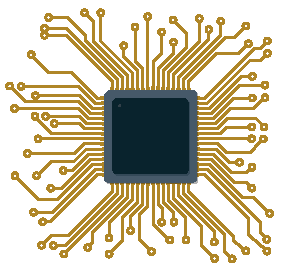
\includegraphics[width=0.3\textwidth]{../resources/chip.pdf}%
}

Around 2004, manufacturers reached what they called the \textit{Power-wall}.
The speed of sequential execution on a processing unit plateaued\ftnt{http://bit.ly/dennard-scaling}.
Therefore, the performance of sequential programming plateaued as well.
They started to arrange transistors into several processing units to keep increasing overall performance efficiency.
Parallel programming became the only option to achieve high concurrency, but the memory isolation it requires limits the productivity.
This \textit{Power-wall} leads to a rupture between efficiency and productivity.

\subsubsection{Conflicting Modularity}

The best practices for productivity in software development advocate to gather features logically into distinct modules.
This modularity allows a developer to understand and contribute to an application one module at a time, instead of understanding the whole application.
It allows to develop and maintain a large code-base by a multitude of developers bringing small, independent contributions.

This modularity avoids a different problem than the isolation required by parallelism.
The former intends to structure code to improve maintainability, while the latter improves performance through parallel execution.
These two organizations are conflicting in the design of the application.
The next paragraph presents the disruptions in the development of a web application implied by this conflict.

\subsubsection{Technological Shift}

% Between the prototyping, and the maturation of a web application, the needs are radically different.
% During the initiation of a web application project, the economical constraint holds on the development productivity.
% The development reactivity is crucial to meet the market needs\ftnt{https://www.cbinsights.com/blog/startup-failure-post-mortem/}.
The development team opt for a popular and accessible language to be productive in the beginning of the project. %  leverage the advantage of its community.
It is only after a certain threshold of user load that the economical constraint on efficiency exceeds the one on productivity.
The development team then shifts to an organization providing parallelism.

This shift brings two risks.
The development team needs to rewrite the code base to adapt it to a completely different paradigm.
The application risks to fail because of this challenge.
And after this shift, the development is less productive.
The development team cannot react as quickly to user feedbacks to adapt the application to the market needs.
The application risks to fall in obsolescence.

The risks implied by this rupture proves that there is economically a need for a solution that continuously follows the evolution of a web application.
The solution proposed in this thesis would allow developers to iterate continuously on the implementation focusing continuously on maintainability and performance.

\subsection{Seamless Web Development}

This thesis is conducted in the frame of a larger work on LiquidIT within the Worldline company.
Worldline develops and hosts real-time streaming Web services.
The company identified that one of its need was to increase the time to market for its products.
Worldline defines LiquidIT as \textit{a concept of flexible and cost-effective IT services that can be provisioned, built and configured in real time, allowing end-to-end financial transparency}.
It precisely intends to provide \textit{business agility, investment-free charging models, flexibility and ease of use}.
This thesis intends to allow the developer to focus solely on business logic, and leave the technical constraints of performance scalability to automated tools.
The objective of this work are to avoid the disruption in development, and provide a seamless development experience.
% They are presented in the next paragraphs.

\subsubsection{Real-Time Streaming Web Services}

This thesis focuses on web applications processing streams of requests from users in soft real-time.
Such applications receive requests from clients through the HTTP protocol and must respond within a finite window of time.
They are generally organized as sequences of tasks to modify the input stream of requests to produce the output stream of responses.
The stream of requests flows through the tasks, and is not stored.
On the other hand, the state of the application remains in memory to impact the future behaviors of the application.
This state might be shared by several tasks within the application, and imply coordination between them.

As presented in the previous section, such applications are often implemented with the event-driven programming model or the pipeline programming model.
This thesis develops an equivalence to map these two models, despite their differences.
% The next section introduces the differences between these two programming models and outlines an equivalence to map these differences.

\subsubsection{Differences Between The Two Models}

Both programming models encapsulate the execution in tasks assured to have an exclusive access to the memory.
However, they use two different models to provide this exclusivity.
Contrary to the pipeline architecture, the event-loop provides a common memory store allowing the best practice of software development to improve maintainability.

These two organizations are incompatible.
And because of economical constraints, this incompatibility implies ruptures in the development.
It represents additional development efforts and important costs.
This thesis argues that it is possible to allow a continuous development between the two organizations, so as to lift these efforts and costs.
To do so, it proposes an equivalence between the two organizations to change from one into the other.
% The argumentation of this possibility is based on an equivalence bridging the two organizations.
It briefly introduces this equivalence in the next paragraph, and details it further in the chapter \ref{chapter4} and \ref{chapter5}.

\subsubsection{Equivalence}

In the beginning of a project, the team focus on productivity, maintainability and evolution, discarding the scalable performance concerns.
The team adopts the event-driven execution model and always sticks with the productive model.
And as the project gather audience and the performance concerns become more and more critical.
The equivalence allows to transform an application expressed in the event-driven execution model into the pipeline execution model.
The generated pipeline expression allows the execution engine to adapt itself to any parallelism of the computing machine, from a single core, to a distributed cluster.
Without giving the productive model up, the development team takes advantage of the different concerns of the tow execution model, performance and maintainability.

\separator

This thesis proposes to provide an equivalence between the two memory models for streaming web applications.
The goal of conciliating these two concerns is not new.
The next chapter presents all the previous results needed to understand this work, up to the latest advances in the field.